\documentclass[a4paper]{article}
\usepackage{cmap}
\usepackage{url}
\usepackage[utf8]{inputenc}
\usepackage[russian]{babel}
\usepackage{graphicx}
\graphicspath{{img/}}
\frenchspacing
\begin{document}
\author{В.\,В.~Бочаров\\\small СПбГУ, OpenCorpora\\\small\tt bocharov@opencorpora.org\and Д.\,В.~Грановский\\\small СПбГУ, OpenCorpora\\\small\tt grand@opencorpora.org\and А.\,В.~Суриков\\\small OpenCorpora\\\small\tt\ ksurent@gmail.com}
\title{Вероятностная модель токенизации в проекте Открытый корпус}
\date{}
\maketitle
\section{Введение}
В проекте <<Открытый Корпус>>~\cite{opcorpora_dialog11}\cite{opcorpora_corpora11} существует ступенчатая процедура добавления текста в корпус. Одним из начальных этапов этой процедуры, как и начальным этапом анализа текста вообще, является токенизация, то есть деление текста на минимальные линейные компоненты~--- токены.

Если судить по количеству публикаций на русском языке, токенизации уделяется не так много внимания по сравнению с более высокоуровневыми этапами анализа, например, морфологическим разбором. При этом вполне очевидно, что токенизация~--- необходимая стадия обработки текста перед его дальнейшим анализом, и ошибки токенизации существенно влияют на работу морфологического парсера; так, авторы статьи~\cite{sharoff_dialog11} решали в т.\,ч. задачу полностью автоматического морфологического анализа текста на русском языке и обнаружили, что наихудшим по качеству компонентом POS-таггера оказался токенизатор, основанный на правилах.

Токенизаторы, основанные на более или менее сложных правилах, являются, по-видимому, самым популярным подходом для русскоязычного текста. В частности, в описании графематического модуля АОТ/Dialing~\cite{sokirko_disser} нет явного указания на правила, но анализ исходного кода~\cite{aot_code} подтверждает, что используется функция, содержательно реализующая именно набор правил. Простейшим набором может быть, например, такой: разделить текст по пробелам; отрезать от каждой получившейся цепочки букв все крайние подцепочки, букв не содержащие.
\section{Проблемы токенизации}
Токенизация в <<Открытом корпусе>> подчиняется нескольким принципам:
\begin{itemize}
\item внутри токена не может быть пробелов,
\item пробел токеном не является,
\item сходные цепочки должны разбиваться единообразно,
все непробельные символы, присутствующие в исходном тексте, сохраняются (о пользе пунктуации для синтаксического анализа см., например,~\cite{okatyev_dialog09}).
\end{itemize}

Кириллические цепочки, как правило, не представляют особенной сложности, за исключением слов, написанных через дефис. Можно выделить некоторые показательные случаи:
\begin{itemize}
\item словарные слова из закрытых классов (какой-нибудь, где-то),
\item произвольные слова с клитиками (мы-то, он-де),
\item приложения (дворник-таджик),
\item составные слова с изменяемой первой частью (кресло-кровать, ракета-носитель),
\item составные слова с неизменяемой первой частью (офис-менеджер, веб-сайт),
\item имена собственные (Жан-Поль, Санкт-Петербург),
\item сокращения, в т.\,ч. с числами (3-й, 24-летний, г-н),
\item названия моделей, событий и т.\,п. (ТУ-154, Евровидение-2011),
\item ошибки (как-бы, то-есть),
\item произвольные авторские комбинации (Тот-кого-нельзя-называть).
\end{itemize}

Некоторые проблемы вызывают и некириллические цепочки. Перечислим самые распространенные, по нашему опыту, спорные случаи:
\begin{itemize}
\item несколько подряд идущих знаков препинания, в частности если эти знаки одинаковые,
\item{<<смайлики>>,}
\item обозначения времени (12:25) и даты (31.12.2011),
\item составные числа (16.3) и дроби (1/4),
\item слова иностранных языков (donne-moi).
\end{itemize}

В каждом из описанных случаев от токенизатора требуется определить, следует ли считать цепочку одним токеном или несколькими. Логика работы здесь, конечно, зависит от требований конкретного проекта (например, в Открытом корпусе принято, что случаи типа \textit{веб-сайт} надо рассматривать как один токен, а случаи типа \textit{Жан-Поль} – как три), но это не очень важно по сравнению с требованием единообразия, которое, как нам кажется, универсально.
\section{Машинное обучение}
На начальном этапе мы также предполагали использовать токенизатор, основанный на правилах, однако довольно быстро выяснилось, что для приемлемого качества токенизации с учетом всевозможных видов токенов количество этих правил должно быть очень велико. В таком случае естественное решение~--- использование машинного обучения.

Процесс добавления текстов в корпус организован так, что результаты работы токенизатора на каждом предложении проверяются вручную. Чем более качественный (в нашем случае~--- близкий к инструкции) результат выдает токенизатор, тем менее трудоемка такая проверка. На начальной стадии (пока для обучения не было данных) все предложения разбивались вручную.

В качестве обучающего множества используются все уже токенизированные предложения корпуса. Каждое предложение представлено в виде пары $(s, T)$, где $s$~--- исходная, нетокенизированная запись предложения (строка), а $T$~--- упорядоченное множество токенов, на которые оно разбито. При этом $s$ всегда можно получить, <<склеив>> все элементы $T$ по порядку, вставляя пробелы, если нужно\footnote{Это утверждение неверно для случаев, когда в тексте имеется несколько пробелов подряд, но нам кажется, что это несущественно, поскольку относится скорее к типографике, чем к языку.}. Следовательно, для каждой позиции $j$ в $s$ можно определить, стоит ли после $j$-го символа граница токенов.

Модель устроена очень просто и представляет собой вероятностный бинарный классификатор: для каждой позиции $j$ вычисляется некоторое количество логических\footnote{Имеется в виду функция, возвращающая одно из двух значений: 0 или 1.} контекстных функций, ее характеризующих (см. ниже), и из результатов вычисления составляется вектор, например, <0, 0, 1, 1, 0, 1>, если функций 6. Накапливая информацию о парах (вектор, наличие границы), после обработки всего обучающего множества получаем для каждого вектора вероятность встретить границу токенов при данных условиях.

Таким образом, применение модели для токенизации текста выглядит так: в каждой позиции текста по тем же правилам, что и при обучении, вычислить вектор двоичных признаков, найти в таблице соответствующую вероятность и решить, достаточно ли эта вероятность высока для постановки границы в данной позиции.

Сходные модели применяются для сегментации русского текста на предложения (\cite{uryupina_dialog08}\cite{kudinov_dialog11}), причем во втором случае предлагается более сложный (и, по-видимому, более эффективный) метод, использующий деревья решений. Нет никаких сомнений, что этот вариант применим и в нашем случае; мы планируем исследовать его в будущем.
\subsection{Контекстные функции}
Большинство контекстных функций работают с минимальным, символьным контекстом~--- левым или правым. Сюда, например, относятся:
\begin{itemize}
\item{<<является ли символ слева буквой кириллицы>>,}
\item{<<является ли символ справа дефисом>>,}
\item{<<является ли символ справа закрывающей скобкой любого вида>> и т.\,п.}
\end{itemize}
Для работы таких функций достаточно информации, содержащейся во входном тексте.

Кроме того, некоторые функции принимают во внимание всю цепочку непробельных символов, внутри которой находятся~--- неважно, оказывается ли она в левом контексте, правом или обоих. Это имеет смысл, когда такая цепочка может оказаться объектом некоторого класса, который подразумевает действие <<всегда разделять>> или <<никогда не разделять>>, например:
\begin{itemize}
\item адресом интернет-ресурса (http://domain.com/a/b/c/page.html) или электронной почты (mail@domain.com),
\item обозначением времени (08:23),
\item словарным словом с дефисом (\textit{по-английски}) и т.\,д.
\end{itemize}

Некоторым из таких функций требуются внешние источники информации~--- например, список всех словарных слов с дефисом или список исключений. Это можно реализовать по-разному; так, в первом случае мы используем запросы к базе данных\footnote{В версии модели для скачивания (см. Заключение) запросы к БД также заменены на читаемый при запуске файл.}, а во втором – простой текстовый файл, загружающийся один раз при запуске программы.

Понятно, что функции могут быть взаимно зависимыми или независимыми. Скажем, функция <<является ли следующий символ пробелом>> и функция <<является ли следующий символ латинской буквой>>, очевидно, зависимы, поскольку символ не может быть одновременно пробелом и латинской буквой. Зависимость функций, в принципе, никак не влияет на модель, но её можно использовать, чтобы составить более короткий вектор без потери информации (закодировав, например, значения четырёх функций двумя битами вместо четырёх), что может быть полезно, если функций много.

На момент написания статьи модель использует 33 функции (в том числе 12 функций, применяемых поочередно к левому и правому символу из минимального контекста), которые~--- за счет зависимости~--- порождают 13-битовый вектор.
\subsection{Порог отсечения}
Принцип работы модели подразумевает, что каждой позиции нетокенизированного текста приписывается некоторая вероятность встретить в этой позиции границу токенов. Очевидно, что для разбиения этого недостаточно, так как необходимо привести каждую вероятность к бинарному значению (разбивать или не разбивать), для чего, в свою очередь, необходимо выбрать порог отсечения~--- т.\,е. значение вероятности, начиная с которого следует считать границу <<достаточно>> вероятной.

Стратегия выбора порога отсечения в целом представляется понятной: необходимо подобрать такое значение, при котором токенизатор будет показывать наибольшую точность работы (в широком смысле) при разбиении предложений обучающего множества (см. раздел <<Оценка качества>>). Это, очевидно, эффективная стратегия в случае, если в дальнейшем предполагается полностью автоматическая работа токенизатора. Однако если по каким-то причинам важнее, допустим, максимизировать полноту за счет точности (иными словами, лучше поставить несколько лишних границ, чем пропустить границу), то порог имеет смысл снизить примерно до 0,01\footnote{По нашему опыту, снижение до 0 даёт побочные эффекты, вызванные шумом (например, опечатками) в исходных данных, см. Рис.~1.}.
\subsection{Оценка качества}
Точность бинарных классификаторов (каковым является токенизатор) общепринято оценивать путем подсчета количества ошибок, которые модель допускает при классификации объектов из некоторого корпуса, при этом ошибки бывают первого рода (ложное срабатывание) и второго рода (пропуск события). В нашем случае ошибка первого рода~--- неверно поставленная граница токенов, а второго~--- пропуск правильной границы. Если рассматривать токенизацию как задачу поиска границ, то можно воспользоваться терминологией информационного поиска и, зная количество ошибок обоих типов, вычислить точность и полноту классификатора.

При оценке мы воспользовались известной техникой кросс-валидации (\textit{cross-validation}, в русскоязычной литературе встречается также перевод <<скользящий контроль>>)\cite{kohavi_crossval}, которая подразумевает, что некоторое размеченное множество примеров (в нашем случае~--- весь доступный корпус, около 700 тыс. токенов) разбивается на $N$ подмножеств, после чего производится $N$ измерений, в каждом из которых очередное подмножество выступает как тестовое, а остальные в совокупности~--- как обучающее. Затем результат усредняется. Мы выбрали $N = 10$: это значение достаточно велико, чтобы усреднение имело смысл, но ещё не столь велико для того, чтобы объём тестового множества стал слишком мал.

Поскольку, как мы уже упоминали, в проекте принято соглашение, что пробел всегда является разделителем токенов, довольно бессмысленно считать все верно расставленные границы до и после пробелов. Поэтому такие случаи были исключены из оценки.

На рис.~1 представлена зависимость точности ($P$), полноты ($R$) и $F_1$-меры от порога отсечения (шаг по оси абсцисс~--- 0,05, кроме того, добавлены значения 0,01 и 0,99).

\begin{figure}[h!]
\center{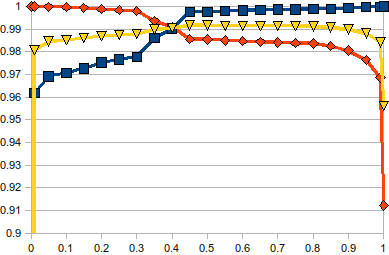
\includegraphics[width=0.7\linewidth]{2012_MIEM_img1.png}}
\caption{}
\end{figure}

Как и следовало ожидать, при увеличении порога отсечения точность монотонно растет, а полнота монотонно убывает. Интересно, что точность при пороге 0 составляет всего около 4\%, а при пороге 0,01 уже более 96\%. Полнота при пороге 1 составляет около 91\%. Максимум $F_1$-меры достигается при пороге около 0,45--0,5 и составляет примерно 99,15\%. Как показывает практика использования токенизатора в Открытом корпусе, это соответствует вполне удовлетворительному качеству токенизации, при котором большинство частотных случаев классифицируется верно. Самые спорные случаи классифицировать иначе, чем вручную, по-видимому, невозможно.

Заметим, что таким образом мы оцениваем, разумеется, не саму вероятностную модель, а конкретную ее реализацию, главным образом~--- набор контекстных функций, а также~--- в некоторой степени~--- качество обучающего множества.

Для сравнения мы проанализировали результат работы простейшего эвристического токенизатора с двумя правилами: всегда разбивать по пробелам, всегда разбивать на границе буквы и не буквы. $F_1$-мера составила около 92\%.
\subsection{Преимущества и недостатки метода}
Описанный метод, в принципе, обладает обычным преимуществом статистических методов: существенно проще~--- по сравнению с моделями, основанными на правилах~--- менять поведение токенизатора на некотором классе случаев (путем изменения набора контекстных функций).

При этом видятся три основных недостатка:
\begin{itemize}
\item невысокая скорость работы как при обучении, так и при классификации, не менее чем линейно зависящая от числа функций,
\item зависимость от качественных (т.\,е. размеченных согласно единому стандарту) обучающих примеров,
\item при собственном стандарте токенизации~--- необходимость изначально существующего размеченного множества примеров для первичного обучения.
\end{itemize}

Очевидно, что для некоторых задач этот метод токенизации не подойдет. Мы предполагаем два сценария, в которых его применение, скорее всего, оправдано:
\begin{itemize}
\item разметка объёмного корпуса, особенно в условиях меняющегося по ходу стандарта токенизации,
\item токенизация текста для задач, где детали стандарта токенизации не очень важны (подразумевается наличие уже обученной модели, см. ниже).
\end{itemize}
\section{Будущая работа}
Качество текущей модели является в целом удовлетворительным. Основным направлением, в котором её можно улучшать, нам видится добавление новых классов сущностей, которые отвечают двум критериям: во-первых, не определяются в рамках существующей модели, во-вторых, при любом осмысленном стандарте токенизации должны трактоваться единообразно. Примером такого класса могут быть <<смайлики>>.

Кроме того, мы планируем исследовать влияние объёма обучающего множества на качество токенизации. There is no data like more data\footnote{Приблизительно переводится как <<чем больше данных, тем лучше>>; известная эвристика машинного обучения, приписываемая разным авторам.}, но в нашем случае огромный (миллионы примеров) объём обучающего множества, во-первых, не всегда достижим, во-вторых, непосредственно влияет на скорость (пере)обучения модели. С другой стороны, если количество контекстных функций (и, соответственно, размерность векторного пространства) растёт, то данные становятся всё более разреженными, что можно компенсировать только увеличением объёма. Таким образом, это вполне насущная проблема.
\section{Заключение}
Описанная модель реализована в виде программного модуля на языке Perl, который доступен для свободного скачивания и применения~\cite{opcorpora_perltok}. Вместе с моделью распространяются данные для неё, т.е. модель уже обучена. К сожалению, на данный момент программный код, реализующий собственно обучение, доступен в менее удобном для использования виде~\cite{opcorpora_tok_code}.
\bibliographystyle{utf8gost780s}
\bibliography{biblio}
\end{document}
